\subsection{Deeper Granular Refinement}
\label{sec:granularityFRESHAlg}
The granularity of the minimal cut sets directly reflect that of the MIVCs. While we eventually may want this algorithm implemented in the safety annex, we chose to begin the refinement in JKind in order to explore granularity from the context of MIVC enumeration. Specific comparisons could be made in terms of the number of MIVCs enumerated, the size of the MIVCs, and the time of analysis. 

The Lustre programming language provides a good formalism for discussion because it is top-level conjunctive, equational, and \emph{referentially transparent}: the behavior or a Lustre program is defined by a system of equations, and any subexpression on the right side of an equation can be extracted and assigned to a fresh variable which is substituted into the original equation without changing the meaning of a program~\cite{Halbwachs91:IEEE,ghassabani_2018}. In this context, we can define a \emph{granular refinement} as an extraction of a subexpression into a new equation assigning a new variable. 

The maximal factorization of the model can be obtained by assigning each instance of a subexpression and each use of an input to its own variable. This results in a \emph{totally decomposed} Lustre model: (1) each computed (non-input) variable is used at most once in the right side of an equation, (2) each equation is either a single operator or a constant expression, and (3) each model input is directly assigned to one or more fresh variables and is not used elsewhere in the model~\cite{ghassabani_2018}.

Ghassabani performed a preliminary analysis on maximally factored models for IVC coverage and found that analysis performed significantly slower for proofs and the \ivcmust algorithm~\cite{ghassabani_2018}. For our purposes in safety analysis, our concern is the guarantees in the Lustre model; therefore, we are able to weaken the factorization performed. To this end, a \emph{partially decomposed} Lustre model has the properties that (1) each computed variable is used at most once in the right side of an equation, and (2) each equation has either a single operator or a literal as the right hand side. The reason we focus on these two properties is because the portions of the model that are of interest are the guarantees (Lustre equations) that constrain the output of a node and any equations these guarantees may reference. We were interested in two main research questions regarding the exploration of granularity refinement: 

\begin{description}
\item[RQ1:] Do the MIVCs generated reflect a more accurate view of which elements of the model support the proof of the safety property? We expect that the additional granularity would provide more exact information regarding which subformulae of a guarantee contribute to proof.

\item [RQ2:] What is the analysis time difference between the nominal model MIVC generation and the decomposed model MIVC generation? Given smaller models with fewer or less complex guarantees, the timing results should not differ greatly, but in a large model with potentially many complex guarantees, the computation time for MIVC generation could increase dramatically. 
 
\end{description}

To explore these questions, we developed an algorithm that performs a partial decomposition of the Lustre model. The logical structure of a formula can be viewed as a tree where nodes are arranged in terms of operator precedence. Clearly, semantic equivalence must be preserved during refactoring and we only want to change the structure (syntax) of the formula. To this end, we isolated branches and subtrees of the structure so that the \aivcalg algorithm can view each subtree of the formula separately. The algorithm recursively travels through a formula tree, assigning each subtree as a fresh variable. Figure~\ref{fig:formulaTree} shows the following formula in tree structure where \textit{lit} refers to a literal:
\begin{gather*}
((((\mathit{lit} \implies \mathit{lit}) \lor \mathit{lit}) \iff \mathit{lit} ) \land (\mathit{lit}  \lor \mathit{lit} )) 
\end{gather*} 

\begin{comment}
\begin{figure}
\begin{center}
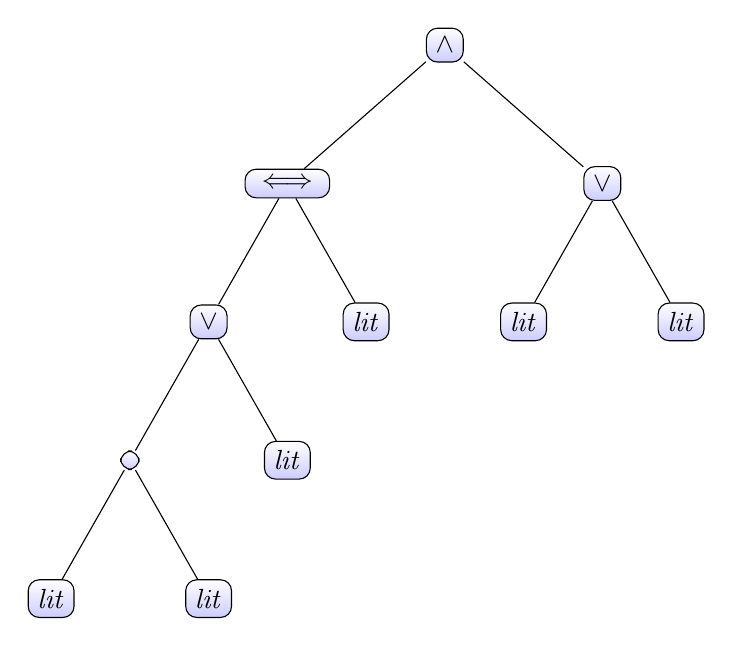
\begin{tikzpicture}[level distance = 5em, every node/.style = {shape=rectangle, rounded corners,
    draw, align=center,
    top color=white, bottom color=blue!20}]]
  \tikzstyle{level 1}=[sibling distance=40mm] 
  \tikzstyle{level 2}=[sibling distance=20mm] 
  \tikzstyle{level 3}=[sibling distance=20mm] 
\node {$\land$} 
    child { node {$\iff$} 
	  child{ node{$\lor$}  
 	    child{node{$\implies$} 
            	 child{ node{\textit{lit}}  } 
	          child{ node{\textit{lit}}  }   
 	    }
 	    child{node{\textit{lit}}}	  
	  }
	  child{ node{\textit{lit}}  }    
    }
    child { node {$\lor$}
      child { node {\textit{lit}} }
      child { node {\textit{lit}} } } ;
\end{tikzpicture}
\end{center}
\caption{Graphical Representation of a Boolean Formula}
\label{fig:formulaTree}
\end{figure}
\end{comment}

\begin{figure}[h!]
\begin{center}
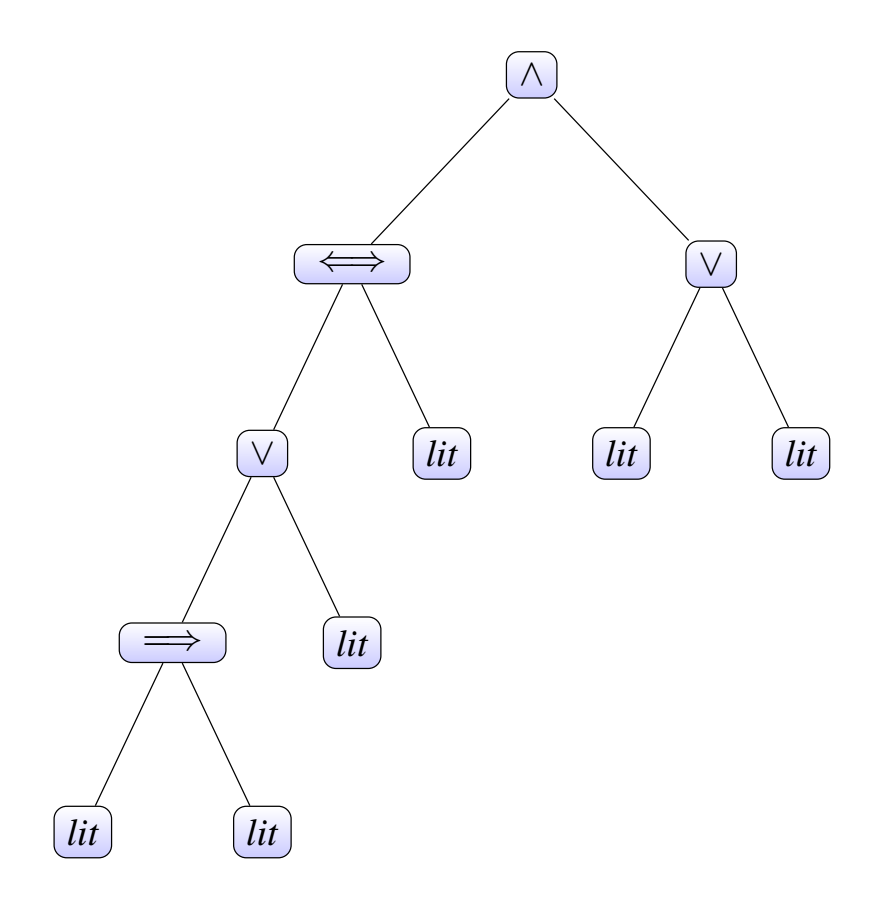
\includegraphics[width=.6\textwidth]{images/treeFormula.png}
\caption{Graphical representation of a Boolean formula} 
\label{fig:formulaTree}
\end{center}
\end{figure} 

As seen in Figure~\ref{fig:formulaTree}, the leaf nodes of the tree are literals; these are the base cases in the recursion. The formula provided as an example has only binary operators; in the algorithm used for refactoring the Lustre equations, unary, binary, and tertiary (if-then-else) operators are handled in a similar fashion.

Each subformula is assigned a fresh variable and added to the equations for the Lustre node. The fresh variables are also assigned to be IVC elements and considered during the \aivcalg algorithm. This is the resulting equation (Figure~\ref{fig:formulaTree}) after refactorization:\\
\texttt{eqn\_name = (FreshVar0);}\\
\texttt{FreshVar0 = (FreshVar1 and FreshVar2);}\\
\texttt{FreshVar1 = (FreshVar3 = lit);}\\
\texttt{FreshVar2 = (lit or lit);}\\
\texttt{FreshVar3 = (FreshVar4 or lit);}\\
\texttt{FreshVar4 = (lit => lit);}

\subsubsection{RQ1}
We present a fictitious monitor component of a system as shown in Figure~\ref{fig:monitorLustre}. There are two components being monitored for validity (components A and B), each of which sends an error indication to the monitor, \texttt{errorCompA} and \texttt{errorCompB}. The monitor calculates  a \texttt{valid} indication if neither error indication is true and when \texttt{output} should be sent. There are two conditions in which the monitor is disabled: when a disable command is explicitly sent or when the system is not in auto mode. The property we wish to show is that the monitor does not calculate both a \texttt{valid} and \texttt{invalid} value simultaneously. 
\begin{figure}[h!]
\begin{center}
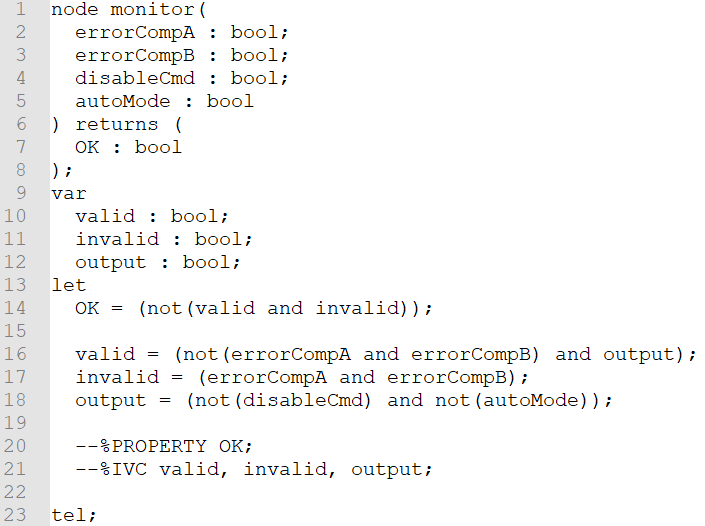
\includegraphics[width=.8\textwidth]{images/monitorLustre.PNG}
\caption{The Lustre Model of a Monitor} 
\label{fig:monitorLustre}
\end{center}
\end{figure} 

The MIVC generated for this property is: $\{$\texttt{valid}, \texttt{invalid}$\}$. Due to the simple nature of this model, it is clear to see that only the error indications from components A and B referenced in equation \texttt{valid} are directly used for the proof of the property, and the branch of \texttt{valid} that references \texttt{output} is not necessary. Since this equation is not sufficiently granular, the MIVC contains the entire \texttt{valid} equation. After performing the refactorization using fresh variables for the model equations, the Lustre code is transformed into what is shown in Figure~\ref{fig:monitorFreshLustre}. 
\begin{figure}[h!]
\begin{center}
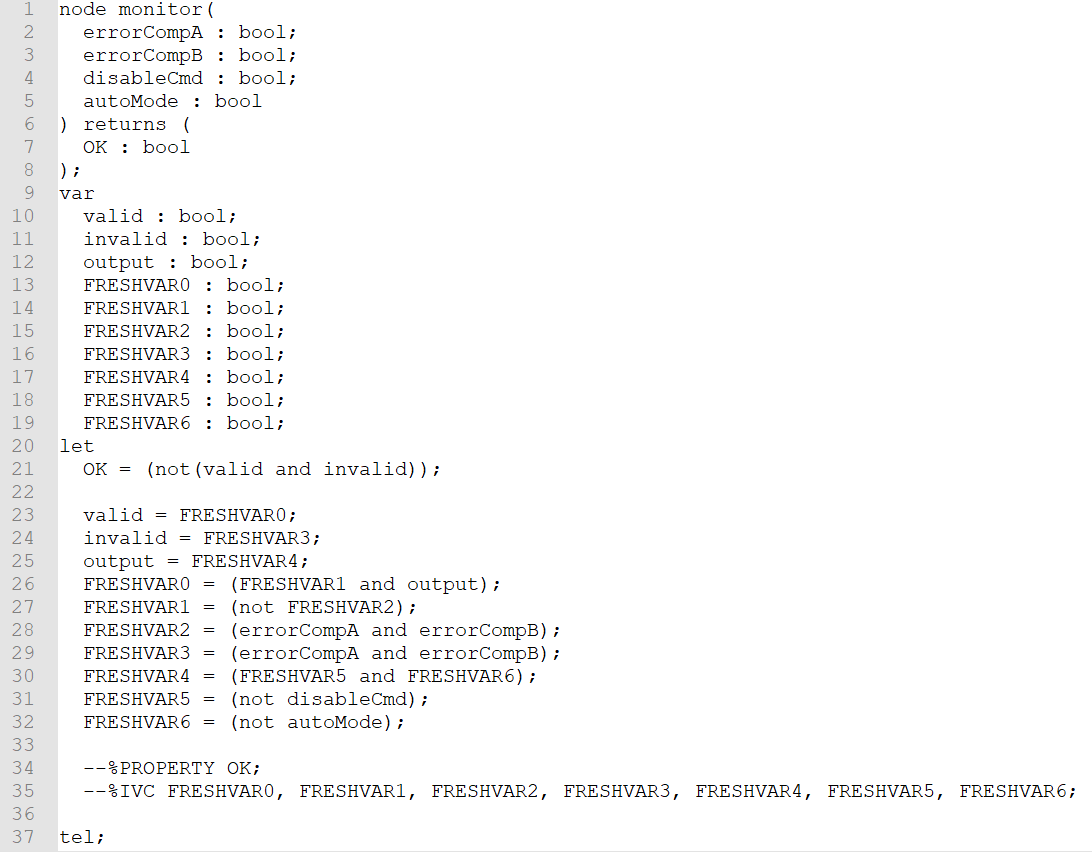
\includegraphics[width=.8\textwidth]{images/monitorFreshLustre.PNG}
\caption{The Lustre Model of a Monitor After Refactorization} \label{fig:monitorFreshLustre}
\end{center}
\end{figure} 

The equations are broken down into their respective subformulae and refactored such that the equations are totally decomposed and semantically equivalent. While this adds a significant number of new variables and equations to the model, the MIVCs generated give more information on the subformulae of the equations necessary for proof. The MIVCs of the refactored model are shown in Figure~\ref{fig:monitorFreshIVCs}. 
\begin{figure}[h!]
\begin{center}
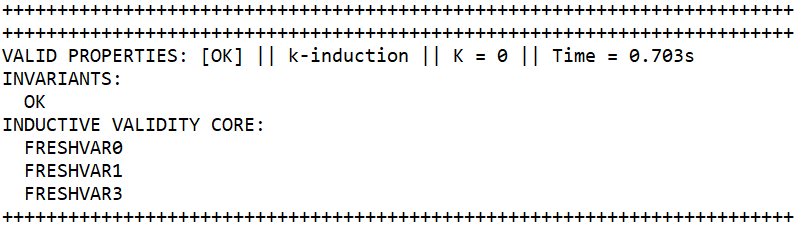
\includegraphics[width=.6\textwidth]{images/monitorFreshIVCs.PNG}
\caption{The MIVC of the Refactored Monitor Model} \label{fig:monitorFreshIVCs}
\end{center}
\end{figure} 

To preserve semantics of the equations during the decomposition, the original equation must be assigned a fresh variable. The MIVC algorithm captures the original equation in \texttt{FRESHVAR0}, but also provides a trace down the branch of the equation that is required for the proof. In this case, it traces down the left side of the original binary equation (\texttt{valid}) and chooses the fresh variable associated with: \texttt{not(errorCompA and errorCompB)}. This correlates to \texttt{FRESHVAR1}. Instead of only providing the equation \texttt{valid} as an MIVC, we see the necessary subformula required for the proof. The third MIVC in this case simply maps back to \texttt{invalid}. 

The MIVCs now provide information on the necessary subformulae of an equation and not only the equation itself. If all branches are required, then all associated fresh variables would be found in those MIVCs. To further explore this question, we also want to see how the sets themselves change after refactorization. To this end, we ran a set of Lustre benchmark models used in previous MIVC enumeration work~\cite{ghassabani_2018} and compared the original MIVC enumerations to the refactored model MIVC results in terms of both number of sets generated and the cardinalities of the sets. In some cases, more MIVCs were generated and in many cases, the MIVCs had greater cardinality. The reason is because every equation that is not assigned to only a literal is refactored and assigned fresh variables. 

\begin{figure}[h!]
\begin{center}
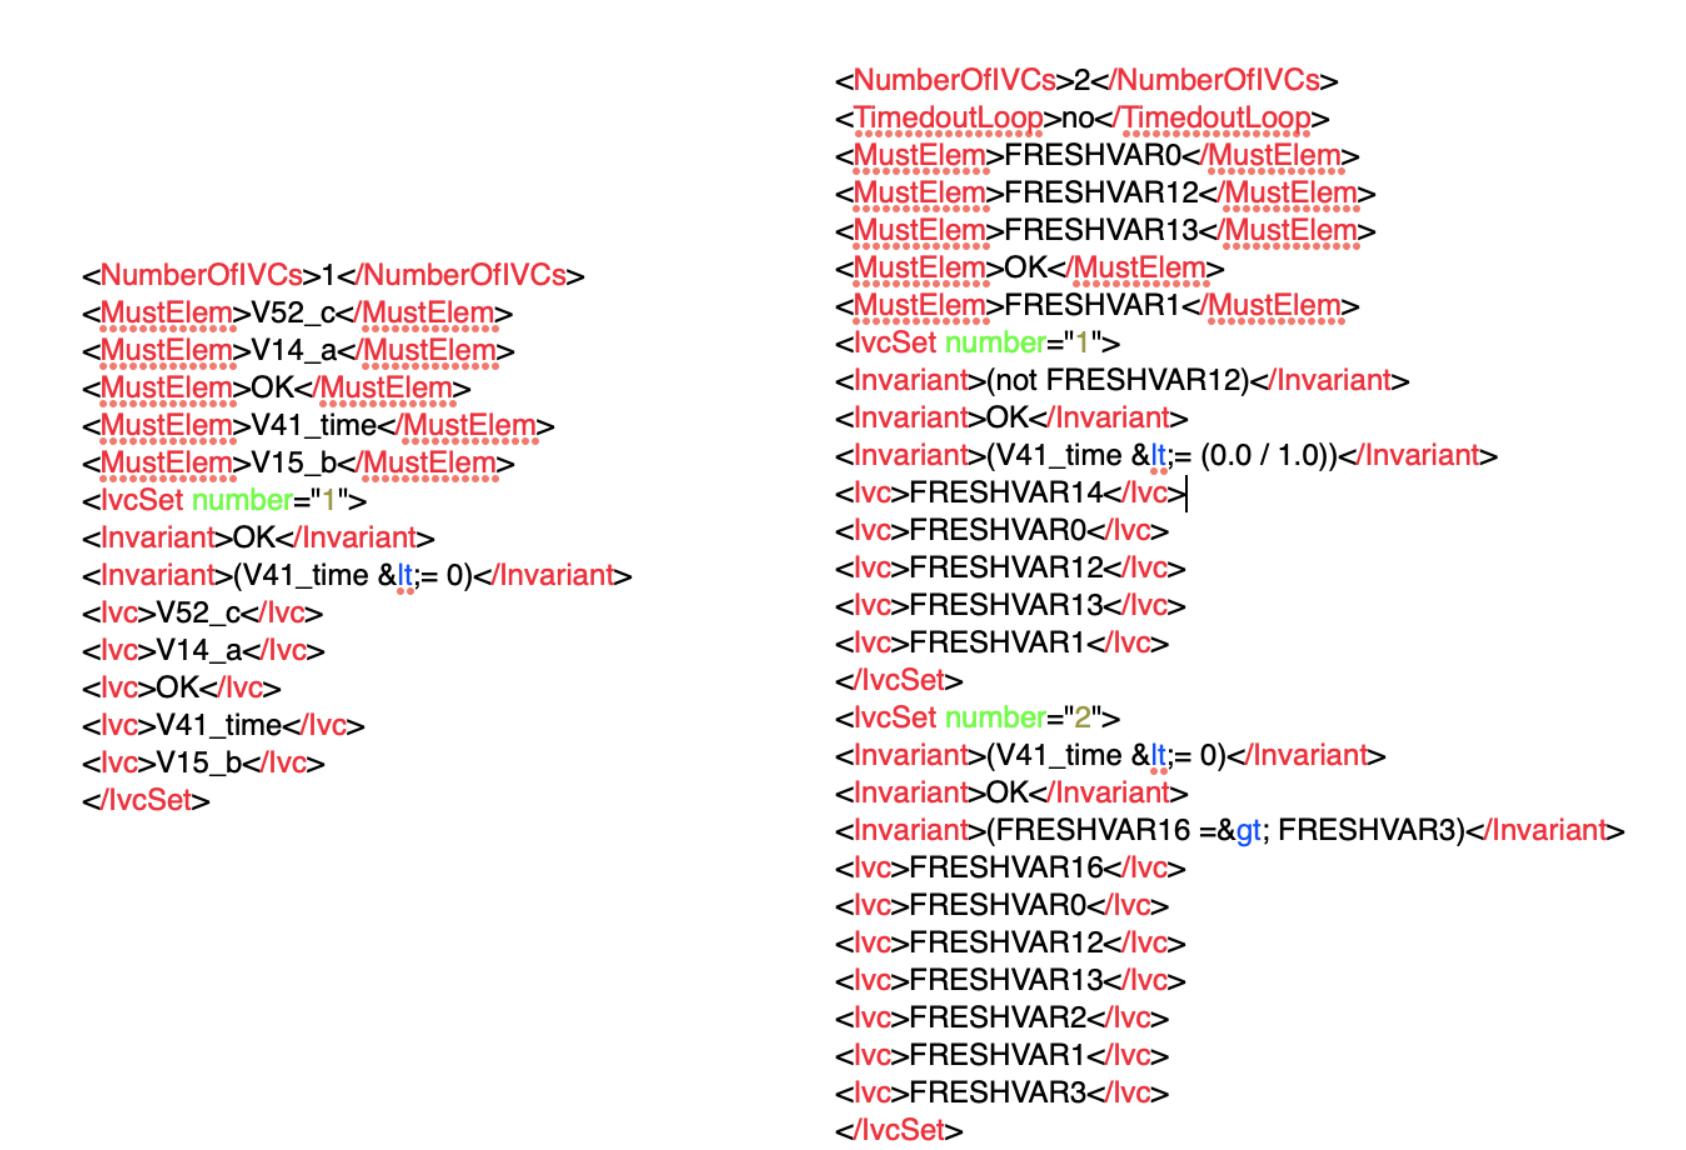
\includegraphics[width=1.0\textwidth]{images/xml_output.png}
\caption{XML MIVC analysis output comparison} 
\label{fig:xml_ivc}
\end{center}
\end{figure}

Figure~\ref{fig:xml_ivc} displays the output of a benchmark model. On the left is the MIVC analysis results for the orginal benchmark model and as a point of comparison, the results for the refactored model are shown on the right. For the original model\footnote{\texttt{\_6counters\_e3\_140\_e8\_149.lus}}, a single IVC of cardinality 5 is enumerated. After refactorization and analysis, the number of MIVCs increased. Depending on the equations necessary for proof of model safety properties, this varies considerably. In some cases, the resulting MIVCs only contain fresh variables corresponding to the original MIVC (cardinality is greater). In other cases, the MIVCs contain fresh variables that describe a subformula of the original results. 

\subsubsection{RQ2}
The refactorization described in the previous section introduces multiple new variables and equations into the Lustre model. While a more exact trace of each equation is possible using this method, the size of the model could grow substantially making the time of analysis unacceptable. We ran a subset of the Lustre benchmark models and compared the time difference between the MIVC enumeration of the refactored models and the MIVC enumeration of the original benchmark models without any refactorization. To use this approach for minimal cut set generation, both the refactorization and the MIVC enumeration must be performed. The total time of the algorithm provided in this chapter and the MIVC collection over the refactored models is used in the time comparison. We used Z3 as a solver and the only IVC elements flagged for consideration were the fresh variables. The timing comparison results are shown in Figure~\ref{fig:granIVC}. 

\begin{figure}[h!]
\begin{center}
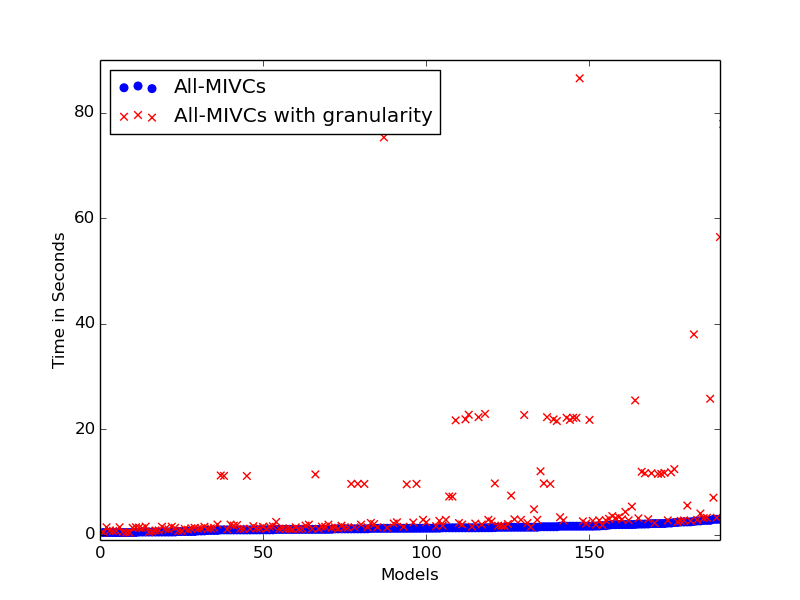
\includegraphics[width=.8\textwidth]{images/granularityIVC2.png}
\caption{Timing comparison for generating MIVCs} 
\label{fig:granIVC}
\end{center}
\end{figure}

For many of the small benchmark models, the time difference between the original and refactored models is not significant. This is likely due to a relatively small number of additional equations inserted into Lustre. Although as can be seen in Figure~\ref{fig:granIVC}, the time of analysis seems to be entirely dependent on the model. All of the models used in this subset of Lustre benchmarks is analyzed using the \aivcalg algorithm in under 6 seconds. The time increase for refactorization varies between the original MIVC time and orders of magnitude higher. When analyzing some of these time intensive models, the reason was clear. The original models contained numerous equations and each equation introduced numerous additional fresh variables into the model.

To introduce a granularity option into the analysis for MIVC enumeration, minimal cut set generation, or other such analyses may provide valuable insight into the model, the specifications, and the faults that contribute to a top level hazard. 

\subsubsection{Future Work for Minimal Cut Sets}
Given the results in RQ2, could more exact minimal cut sets be produced from the MIVCs? If changes are reflected in the MIVC sets, then we will see corresponding changes in the minimal cut sets as shown in the preliminary investigation of Section~\ref{sec:granularityANDAlg}. This Would provide more exact safety analysis artifacts and additional insight into the specifications and how they impact the analysis results.

The method used in this algorithm provides all fresh variables to the MIVC algorithm. The results seen in the MIVCs reflect a branch of the Boolean equation. The transformation from MIVCs to minimal cut sets include a hitting set algorithm. Given the IVC results of this granularity algorithm, the hitting sets would split the branch shown in the MIVC such that the semantics of results would no longer be sound. In order to use these MIVCs for minimal cut set generation, he branch of a formula in an MIVC would need to be inlined before the hitting sets were computed. At that point, the single formula/branch could be used in the hitting set algorithm without loss of meaning. 

After this processing, the minimal cut sets could be found by mapping the subformula to a fault that violates the output referenced in that subformula. Further work is required to implement this approach, but given the preliminary findings of this exploration, this approach is promising to provide insight into model specifications, subformula necessary for proof, and more exact minimal cut sets. 






